% Options for packages loaded elsewhere
\PassOptionsToPackage{unicode}{hyperref}
\PassOptionsToPackage{hyphens}{url}
%
\documentclass[
  11pt,
]{article}
\usepackage{amsmath,amssymb}
\usepackage{iftex}
\ifPDFTeX
  \usepackage[T1]{fontenc}
  \usepackage[utf8]{inputenc}
  \usepackage{textcomp} % provide euro and other symbols
\else % if luatex or xetex
  \usepackage{unicode-math} % this also loads fontspec
  \defaultfontfeatures{Scale=MatchLowercase}
  \defaultfontfeatures[\rmfamily]{Ligatures=TeX,Scale=1}
\fi
\usepackage{lmodern}
\ifPDFTeX\else
  % xetex/luatex font selection
\fi
% Use upquote if available, for straight quotes in verbatim environments
\IfFileExists{upquote.sty}{\usepackage{upquote}}{}
\IfFileExists{microtype.sty}{% use microtype if available
  \usepackage[]{microtype}
  \UseMicrotypeSet[protrusion]{basicmath} % disable protrusion for tt fonts
}{}
\makeatletter
\@ifundefined{KOMAClassName}{% if non-KOMA class
  \IfFileExists{parskip.sty}{%
    \usepackage{parskip}
  }{% else
    \setlength{\parindent}{0pt}
    \setlength{\parskip}{6pt plus 2pt minus 1pt}}
}{% if KOMA class
  \KOMAoptions{parskip=half}}
\makeatother
\usepackage{xcolor}
\usepackage[margin=1in]{geometry}
\usepackage{color}
\usepackage{fancyvrb}
\newcommand{\VerbBar}{|}
\newcommand{\VERB}{\Verb[commandchars=\\\{\}]}
\DefineVerbatimEnvironment{Highlighting}{Verbatim}{commandchars=\\\{\}}
% Add ',fontsize=\small' for more characters per line
\usepackage{framed}
\definecolor{shadecolor}{RGB}{248,248,248}
\newenvironment{Shaded}{\begin{snugshade}}{\end{snugshade}}
\newcommand{\AlertTok}[1]{\textcolor[rgb]{0.94,0.16,0.16}{#1}}
\newcommand{\AnnotationTok}[1]{\textcolor[rgb]{0.56,0.35,0.01}{\textbf{\textit{#1}}}}
\newcommand{\AttributeTok}[1]{\textcolor[rgb]{0.13,0.29,0.53}{#1}}
\newcommand{\BaseNTok}[1]{\textcolor[rgb]{0.00,0.00,0.81}{#1}}
\newcommand{\BuiltInTok}[1]{#1}
\newcommand{\CharTok}[1]{\textcolor[rgb]{0.31,0.60,0.02}{#1}}
\newcommand{\CommentTok}[1]{\textcolor[rgb]{0.56,0.35,0.01}{\textit{#1}}}
\newcommand{\CommentVarTok}[1]{\textcolor[rgb]{0.56,0.35,0.01}{\textbf{\textit{#1}}}}
\newcommand{\ConstantTok}[1]{\textcolor[rgb]{0.56,0.35,0.01}{#1}}
\newcommand{\ControlFlowTok}[1]{\textcolor[rgb]{0.13,0.29,0.53}{\textbf{#1}}}
\newcommand{\DataTypeTok}[1]{\textcolor[rgb]{0.13,0.29,0.53}{#1}}
\newcommand{\DecValTok}[1]{\textcolor[rgb]{0.00,0.00,0.81}{#1}}
\newcommand{\DocumentationTok}[1]{\textcolor[rgb]{0.56,0.35,0.01}{\textbf{\textit{#1}}}}
\newcommand{\ErrorTok}[1]{\textcolor[rgb]{0.64,0.00,0.00}{\textbf{#1}}}
\newcommand{\ExtensionTok}[1]{#1}
\newcommand{\FloatTok}[1]{\textcolor[rgb]{0.00,0.00,0.81}{#1}}
\newcommand{\FunctionTok}[1]{\textcolor[rgb]{0.13,0.29,0.53}{\textbf{#1}}}
\newcommand{\ImportTok}[1]{#1}
\newcommand{\InformationTok}[1]{\textcolor[rgb]{0.56,0.35,0.01}{\textbf{\textit{#1}}}}
\newcommand{\KeywordTok}[1]{\textcolor[rgb]{0.13,0.29,0.53}{\textbf{#1}}}
\newcommand{\NormalTok}[1]{#1}
\newcommand{\OperatorTok}[1]{\textcolor[rgb]{0.81,0.36,0.00}{\textbf{#1}}}
\newcommand{\OtherTok}[1]{\textcolor[rgb]{0.56,0.35,0.01}{#1}}
\newcommand{\PreprocessorTok}[1]{\textcolor[rgb]{0.56,0.35,0.01}{\textit{#1}}}
\newcommand{\RegionMarkerTok}[1]{#1}
\newcommand{\SpecialCharTok}[1]{\textcolor[rgb]{0.81,0.36,0.00}{\textbf{#1}}}
\newcommand{\SpecialStringTok}[1]{\textcolor[rgb]{0.31,0.60,0.02}{#1}}
\newcommand{\StringTok}[1]{\textcolor[rgb]{0.31,0.60,0.02}{#1}}
\newcommand{\VariableTok}[1]{\textcolor[rgb]{0.00,0.00,0.00}{#1}}
\newcommand{\VerbatimStringTok}[1]{\textcolor[rgb]{0.31,0.60,0.02}{#1}}
\newcommand{\WarningTok}[1]{\textcolor[rgb]{0.56,0.35,0.01}{\textbf{\textit{#1}}}}
\usepackage{graphicx}
\makeatletter
\def\maxwidth{\ifdim\Gin@nat@width>\linewidth\linewidth\else\Gin@nat@width\fi}
\def\maxheight{\ifdim\Gin@nat@height>\textheight\textheight\else\Gin@nat@height\fi}
\makeatother
% Scale images if necessary, so that they will not overflow the page
% margins by default, and it is still possible to overwrite the defaults
% using explicit options in \includegraphics[width, height, ...]{}
\setkeys{Gin}{width=\maxwidth,height=\maxheight,keepaspectratio}
% Set default figure placement to htbp
\makeatletter
\def\fps@figure{htbp}
\makeatother
\setlength{\emergencystretch}{3em} % prevent overfull lines
\providecommand{\tightlist}{%
  \setlength{\itemsep}{0pt}\setlength{\parskip}{0pt}}
\setcounter{secnumdepth}{5}
\usepackage[font=footnotesize]{caption}
\usepackage{dirtytalk}
\usepackage{booktabs}
\usepackage{tabulary}
\usepackage{enumitem}
\usepackage{lmodern}
\usepackage[T1]{fontenc}
\usepackage{tikz}
\ifLuaTeX
  \usepackage{selnolig}  % disable illegal ligatures
\fi
\IfFileExists{bookmark.sty}{\usepackage{bookmark}}{\usepackage{hyperref}}
\IfFileExists{xurl.sty}{\usepackage{xurl}}{} % add URL line breaks if available
\urlstyle{same}
\hypersetup{
  pdftitle={Code of Fallacies in the Global Water Crisis statistics},
  pdfauthor={Arnald Puy},
  hidelinks,
  pdfcreator={LaTeX via pandoc}}

\title{Code of Fallacies in the Global Water Crisis statistics}
\usepackage{etoolbox}
\makeatletter
\providecommand{\subtitle}[1]{% add subtitle to \maketitle
  \apptocmd{\@title}{\par {\large #1 \par}}{}{}
}
\makeatother
\subtitle{R code}
\author{Arnald Puy}
\date{}

\begin{document}
\maketitle

{
\setcounter{tocdepth}{2}
\tableofcontents
}
\newpage

\begin{Shaded}
\begin{Highlighting}[]
\CommentTok{\# PRELIMINARY {-}{-}{-}{-}{-}{-}{-}{-}{-}{-}{-}{-}{-}{-}{-}{-}{-}{-}{-}{-}{-}{-}{-}{-}{-}{-}{-}{-}{-}{-}{-}{-}{-}{-}{-}{-}{-}{-}{-}{-}{-}{-}{-}{-}{-}{-}{-}{-}{-}{-}{-}{-}{-}{-}{-}{-}{-}{-}{-}{-}{-}{-}{-}{-}{-}}

\NormalTok{sensobol}\SpecialCharTok{::}\FunctionTok{load\_packages}\NormalTok{(}\FunctionTok{c}\NormalTok{(}\StringTok{"sensobol"}\NormalTok{, }\StringTok{"tidyverse"}\NormalTok{, }\StringTok{"data.table"}\NormalTok{, }\StringTok{"cowplot"}\NormalTok{, }
                          \StringTok{"scales"}\NormalTok{, }\StringTok{"rvest"}\NormalTok{, }\StringTok{"janitor"}\NormalTok{, }\StringTok{"fitdistrplus"}\NormalTok{, }\StringTok{"wesanderson"}\NormalTok{))}
\NormalTok{theme\_AP }\OtherTok{\textless{}{-}} \ControlFlowTok{function}\NormalTok{() \{}
  \FunctionTok{theme\_bw}\NormalTok{() }\SpecialCharTok{+}
    \FunctionTok{theme}\NormalTok{(}\AttributeTok{panel.grid.major =} \FunctionTok{element\_blank}\NormalTok{(),}
          \AttributeTok{panel.grid.minor =} \FunctionTok{element\_blank}\NormalTok{(),}
          \AttributeTok{legend.background =} \FunctionTok{element\_rect}\NormalTok{(}\AttributeTok{fill =} \StringTok{"transparent"}\NormalTok{,}
                                           \AttributeTok{color =} \ConstantTok{NA}\NormalTok{),}
          \AttributeTok{legend.margin=}\FunctionTok{margin}\NormalTok{(}\DecValTok{0}\NormalTok{, }\DecValTok{0}\NormalTok{, }\DecValTok{0}\NormalTok{, }\DecValTok{0}\NormalTok{),}
          \AttributeTok{legend.box.margin=}\FunctionTok{margin}\NormalTok{(}\SpecialCharTok{{-}}\DecValTok{5}\NormalTok{,}\SpecialCharTok{{-}}\DecValTok{5}\NormalTok{,}\SpecialCharTok{{-}}\DecValTok{5}\NormalTok{,}\SpecialCharTok{{-}}\DecValTok{5}\NormalTok{), }
          \AttributeTok{legend.key =} \FunctionTok{element\_rect}\NormalTok{(}\AttributeTok{fill =} \StringTok{"transparent"}\NormalTok{,}
                                    \AttributeTok{color =} \ConstantTok{NA}\NormalTok{), }
          \AttributeTok{strip.background =} \FunctionTok{element\_rect}\NormalTok{(}\AttributeTok{fill =} \StringTok{"white"}\NormalTok{), }
          \AttributeTok{axis.title =} \FunctionTok{element\_text}\NormalTok{(}\AttributeTok{size =} \DecValTok{9}\NormalTok{), }
          \AttributeTok{legend.text =} \FunctionTok{element\_text}\NormalTok{(}\AttributeTok{size =} \DecValTok{9}\NormalTok{), }
          \AttributeTok{legend.title =} \FunctionTok{element\_text}\NormalTok{(}\AttributeTok{size =} \DecValTok{9}\NormalTok{), }
          \AttributeTok{legend.key.width =} \FunctionTok{unit}\NormalTok{(}\FloatTok{0.3}\NormalTok{, }\StringTok{"cm"}\NormalTok{),}
          \AttributeTok{legend.key.height =} \FunctionTok{unit}\NormalTok{(}\FloatTok{0.3}\NormalTok{, }\StringTok{"cm"}\NormalTok{))}
\NormalTok{\}}

\DocumentationTok{\#\# {-}{-}{-}{-}calculations, warning=FALSE{-}{-}{-}{-}{-}{-}{-}{-}{-}{-}{-}{-}{-}{-}{-}{-}{-}{-}{-}{-}{-}{-}{-}{-}{-}{-}{-}{-}{-}{-}{-}{-}{-}{-}{-}{-}{-}{-}{-}{-}{-}{-}{-}{-}{-}{-}{-}{-}{-}{-}{-}{-}{-}{-}{-}{-}{-}{-}{-}}

\CommentTok{\# SETTINGS \#\#\#\#\#\#\#\#\#\#\#\#\#\#\#\#\#\#\#\#\#\#\#\#\#\#\#\#\#\#\#\#\#\#\#\#\#\#\#\#\#\#\#\#\#\#\#\#\#\#\#\#\#\#\#\#\#\#\#\#\#\#\#\#\#\#\#\#\#}

\CommentTok{\# Values used in the paper}
\NormalTok{precipitation\_estimate }\OtherTok{\textless{}{-}} \DecValTok{120000}
\NormalTok{precipitation\_min }\OtherTok{\textless{}{-}}\NormalTok{ precipitation\_estimate }\SpecialCharTok{{-}}\NormalTok{ (precipitation\_estimate }\SpecialCharTok{*} \FloatTok{0.1}\NormalTok{)}
\NormalTok{precipitation\_max }\OtherTok{\textless{}{-}}\NormalTok{ precipitation\_estimate }\SpecialCharTok{+}\NormalTok{ (precipitation\_estimate }\SpecialCharTok{*} \FloatTok{0.1}\NormalTok{)}

\NormalTok{land\_runoff\_estimate }\OtherTok{\textless{}{-}} \DecValTok{46000}
\NormalTok{land\_runoff\_min }\OtherTok{\textless{}{-}}\NormalTok{ land\_runoff\_estimate }\SpecialCharTok{{-}}\NormalTok{ (land\_runoff\_estimate  }\SpecialCharTok{*} \FloatTok{0.1}\NormalTok{)}
\NormalTok{land\_runoff\_max }\OtherTok{\textless{}{-}}\NormalTok{ land\_runoff\_estimate }\SpecialCharTok{+}\NormalTok{ (land\_runoff\_estimate  }\SpecialCharTok{*} \FloatTok{0.1}\NormalTok{)}

\CommentTok{\# RETRIEVE DATA FOR KILOCALORIES \#\#\#\#\#\#\#\#\#\#\#\#\#\#\#\#\#\#\#\#\#\#\#\#\#\#\#\#\#\#\#\#\#\#\#\#\#\#\#\#\#\#\#\#\#\#\#}

\CommentTok{\# Read the HTML content of the website }
\NormalTok{webpage }\OtherTok{\textless{}{-}} \FunctionTok{read\_html}\NormalTok{(}\StringTok{"https://en.wikipedia.org/wiki/List\_of\_countries\_by\_food\_energy\_intake\#cite\_note{-}8"}\NormalTok{) }

\CommentTok{\# Select the table using CSS selector }
\NormalTok{table\_node }\OtherTok{\textless{}{-}} \FunctionTok{html\_nodes}\NormalTok{(webpage, }\StringTok{"table"}\NormalTok{) }

\CommentTok{\# Extract the table content }
\NormalTok{table\_content }\OtherTok{\textless{}{-}} \FunctionTok{data.table}\NormalTok{(}\FunctionTok{html\_table}\NormalTok{(table\_node, }\AttributeTok{header =} \ConstantTok{TRUE}\NormalTok{)[[}\DecValTok{1}\NormalTok{]]) }\SpecialCharTok{\%\textgreater{}\%}
  \FunctionTok{row\_to\_names}\NormalTok{(}\AttributeTok{row\_number =} \DecValTok{1}\NormalTok{)}

\CommentTok{\# Arrange and clean columns {-}{-}{-}{-}{-}{-}{-}{-}{-}{-}{-}{-}{-}{-}{-}{-}{-}{-}{-}{-}{-}{-}{-}{-}{-}{-}{-}{-}{-}{-}{-}{-}{-}{-}{-}{-}{-}{-}{-}{-}{-}{-}{-}{-}{-}{-}{-}{-}{-}{-}{-}{-}}
\NormalTok{old\_colnames }\OtherTok{\textless{}{-}} \FunctionTok{colnames}\NormalTok{(table\_content)}
\NormalTok{new\_colnames }\OtherTok{\textless{}{-}} \FunctionTok{c}\NormalTok{(}\StringTok{"rank"}\NormalTok{, }\StringTok{"country"}\NormalTok{, }\StringTok{"kcal"}\NormalTok{, }\StringTok{"year"}\NormalTok{)}
\FunctionTok{setnames}\NormalTok{(table\_content, old\_colnames, new\_colnames)}
\NormalTok{table\_content[, kcal}\SpecialCharTok{:=} \FunctionTok{as.numeric}\NormalTok{(}\FunctionTok{gsub}\NormalTok{(}\StringTok{","}\NormalTok{, }\StringTok{""}\NormalTok{, kcal))]}

\CommentTok{\# Check best distribution}
\NormalTok{fg }\OtherTok{\textless{}{-}} \FunctionTok{fitdist}\NormalTok{(table\_content}\SpecialCharTok{$}\NormalTok{kcal, }\StringTok{"gamma"}\NormalTok{)}
\NormalTok{fln }\OtherTok{\textless{}{-}} \FunctionTok{fitdist}\NormalTok{(table\_content}\SpecialCharTok{$}\NormalTok{kcal, }\StringTok{"lnorm"}\NormalTok{)}
\NormalTok{fw }\OtherTok{\textless{}{-}} \FunctionTok{fitdist}\NormalTok{(table\_content}\SpecialCharTok{$}\NormalTok{kcal, }\StringTok{"weibull"}\NormalTok{)}

\CommentTok{\# Plot goodness of fit {-}{-}{-}{-}{-}{-}{-}{-}{-}{-}{-}{-}{-}{-}{-}{-}{-}{-}{-}{-}{-}{-}{-}{-}{-}{-}{-}{-}{-}{-}{-}{-}{-}{-}{-}{-}{-}{-}{-}{-}{-}{-}{-}{-}{-}{-}{-}{-}{-}{-}{-}{-}{-}{-}{-}{-}{-}}
\FunctionTok{par}\NormalTok{(}\AttributeTok{mfrow =} \FunctionTok{c}\NormalTok{(}\DecValTok{2}\NormalTok{, }\DecValTok{2}\NormalTok{))}
\NormalTok{plot.legend }\OtherTok{\textless{}{-}} \FunctionTok{c}\NormalTok{(}\StringTok{"gamma"}\NormalTok{, }\StringTok{"lognormal"}\NormalTok{,}\StringTok{"weibull"}\NormalTok{)}
\FunctionTok{denscomp}\NormalTok{(}\FunctionTok{list}\NormalTok{(fg, fln, fw), }\AttributeTok{legendtext =}\NormalTok{ plot.legend)}
\FunctionTok{qqcomp}\NormalTok{(}\FunctionTok{list}\NormalTok{(fg, fln, fw), }\AttributeTok{legendtext =}\NormalTok{ plot.legend)}
\FunctionTok{cdfcomp}\NormalTok{(}\FunctionTok{list}\NormalTok{(fg, fln, fw), }\AttributeTok{legendtext =}\NormalTok{ plot.legend)}
\FunctionTok{ppcomp}\NormalTok{(}\FunctionTok{list}\NormalTok{(fg, fln, fw), }\AttributeTok{legendtext =}\NormalTok{ plot.legend)}
\end{Highlighting}
\end{Shaded}

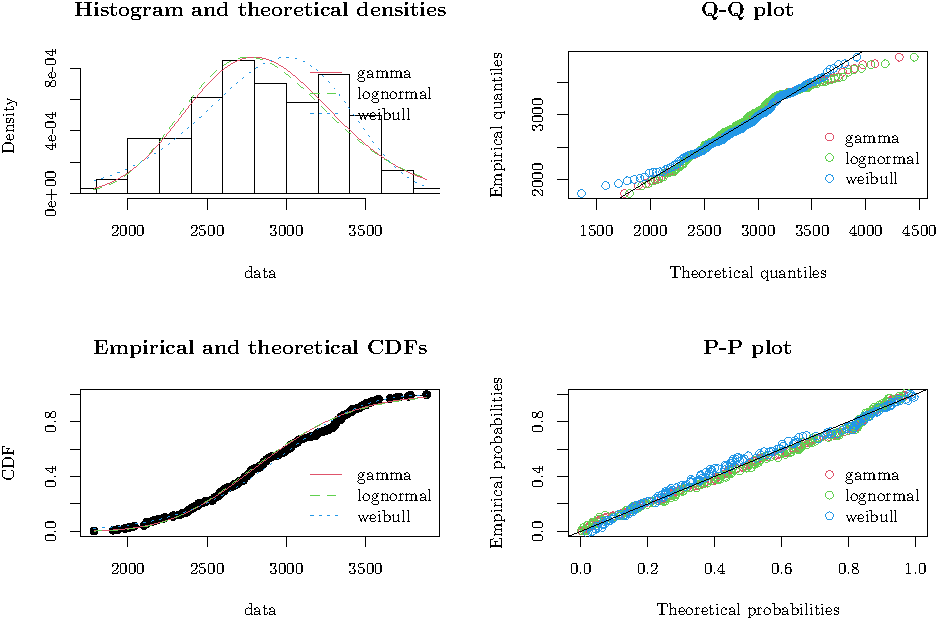
\includegraphics{code_fallacies_water_crisis_files/figure-latex/all_model-1.pdf}

\begin{Shaded}
\begin{Highlighting}[]
\CommentTok{\# Opt for truncated weibull {-}{-}{-}{-}{-}{-}{-}{-}{-}{-}{-}{-}{-}{-}{-}{-}{-}{-}{-}{-}{-}{-}{-}{-}{-}{-}{-}{-}{-}{-}{-}{-}{-}{-}{-}{-}{-}{-}{-}{-}{-}{-}{-}{-}{-}{-}{-}{-}{-}{-}{-}{-}}
\NormalTok{shape }\OtherTok{\textless{}{-}}\NormalTok{ fw}\SpecialCharTok{$}\NormalTok{estimate[[}\DecValTok{1}\NormalTok{]]}
\NormalTok{scale }\OtherTok{\textless{}{-}}\NormalTok{ fw}\SpecialCharTok{$}\NormalTok{estimate[[}\DecValTok{2}\NormalTok{]]}
\NormalTok{minimum }\OtherTok{\textless{}{-}} \FunctionTok{min}\NormalTok{(table\_content}\SpecialCharTok{$}\NormalTok{kcal)}
\NormalTok{maximum }\OtherTok{\textless{}{-}} \FunctionTok{max}\NormalTok{(table\_content}\SpecialCharTok{$}\NormalTok{kcal)}
\NormalTok{weibull\_dist }\OtherTok{\textless{}{-}} \FunctionTok{sapply}\NormalTok{(}\FunctionTok{c}\NormalTok{(minimum, maximum), }\ControlFlowTok{function}\NormalTok{(x)}
  \FunctionTok{pweibull}\NormalTok{(x, }\AttributeTok{shape =}\NormalTok{ shape, }\AttributeTok{scale =}\NormalTok{ scale))}

\CommentTok{\# SAMPLE MATRIX \#\#\#\#\#\#\#\#\#\#\#\#\#\#\#\#\#\#\#\#\#\#\#\#\#\#\#\#\#\#\#\#\#\#\#\#\#\#\#\#\#\#\#\#\#\#\#\#\#\#\#\#\#\#\#\#\#\#\#\#\#\#\#\#}

\NormalTok{N }\OtherTok{\textless{}{-}} \DecValTok{2}\SpecialCharTok{\^{}}\DecValTok{13}
\NormalTok{params }\OtherTok{\textless{}{-}} \FunctionTok{c}\NormalTok{(}\StringTok{"precipitation"}\NormalTok{, }\StringTok{"et\_crops"}\NormalTok{, }\StringTok{"et\_vegetation"}\NormalTok{, }\StringTok{"global\_consumption"}\NormalTok{, }
            \StringTok{"planetary\_boundary"}\NormalTok{, }\StringTok{"W\_g"}\NormalTok{, }\StringTok{"W\_i"}\NormalTok{, }\StringTok{"F\_i"}\NormalTok{, }\StringTok{"F\_u"}\NormalTok{, }\StringTok{"$k$"}\NormalTok{, }\StringTok{"F\_b"}\NormalTok{, }
            \StringTok{"$F\_m$"}\NormalTok{, }\StringTok{"$F\_\{m\_w\}$"}\NormalTok{, }\StringTok{"$F\_\{v\_w\}$"}\NormalTok{)}

\NormalTok{mat }\OtherTok{\textless{}{-}} \FunctionTok{sobol\_matrices}\NormalTok{(}\AttributeTok{N =}\NormalTok{ N, }\AttributeTok{params =}\NormalTok{ params)}

\CommentTok{\# Uncertain parameters in Figure 1 {-}{-}{-}{-}{-}{-}{-}{-}{-}{-}{-}{-}{-}{-}{-}{-}{-}{-}{-}{-}{-}{-}{-}{-}{-}{-}{-}{-}{-}{-}{-}{-}{-}{-}{-}{-}{-}{-}{-}{-}{-}{-}{-}{-}{-}}
\NormalTok{mat[, }\StringTok{"precipitation"}\NormalTok{] }\OtherTok{\textless{}{-}} \FunctionTok{qunif}\NormalTok{(mat[, }\StringTok{"precipitation"}\NormalTok{], precipitation\_min, precipitation\_max)}
\NormalTok{mat[, }\StringTok{"et\_crops"}\NormalTok{] }\OtherTok{\textless{}{-}} \FunctionTok{qunif}\NormalTok{(mat[, }\StringTok{"et\_crops"}\NormalTok{], }\DecValTok{5200}\NormalTok{, }\DecValTok{5800}\NormalTok{)}
\NormalTok{mat[, }\StringTok{"et\_vegetation"}\NormalTok{] }\OtherTok{\textless{}{-}} \FunctionTok{qunif}\NormalTok{(mat[, }\StringTok{"et\_vegetation"}\NormalTok{], }\DecValTok{68200}\NormalTok{, }\DecValTok{68800}\NormalTok{)}
\NormalTok{mat[, }\StringTok{"global\_consumption"}\NormalTok{] }\OtherTok{\textless{}{-}} \FunctionTok{qunif}\NormalTok{(mat[, }\StringTok{"global\_consumption"}\NormalTok{], }\DecValTok{3391}\NormalTok{, }\DecValTok{5349}\NormalTok{)}
\NormalTok{mat[, }\StringTok{"planetary\_boundary"}\NormalTok{] }\OtherTok{\textless{}{-}} \FunctionTok{qunif}\NormalTok{(mat[, }\StringTok{"planetary\_boundary"}\NormalTok{], }\DecValTok{4000}\NormalTok{, }\DecValTok{6000}\NormalTok{)}

\CommentTok{\# Uncertain parameters for water exceedance in 2023 {-}{-}{-}{-}{-}{-}{-}{-}{-}{-}{-}{-}{-}{-}{-}{-}{-}{-}{-}{-}{-}{-}{-}{-}{-}{-}{-}{-}}

\CommentTok{\# Estimates groundwater consumption}
\NormalTok{mat[, }\StringTok{"W\_g"}\NormalTok{] }\OtherTok{\textless{}{-}} \FunctionTok{qunif}\NormalTok{(mat[, }\StringTok{"W\_g"}\NormalTok{], }\DecValTok{84}\NormalTok{, }\DecValTok{304}\NormalTok{) }

\CommentTok{\# estimates irrigation water consumption}
\NormalTok{mat[, }\StringTok{"W\_i"}\NormalTok{] }\OtherTok{\textless{}{-}} \FunctionTok{qunif}\NormalTok{(mat[, }\StringTok{"W\_i"}\NormalTok{], }\DecValTok{1083}\NormalTok{, }\DecValTok{1550}\NormalTok{) }

\CommentTok{\# fraction of irrigation over total water consumption}
\NormalTok{mat[, }\StringTok{"F\_i"}\NormalTok{] }\OtherTok{\textless{}{-}} \FunctionTok{qunif}\NormalTok{(mat[, }\StringTok{"F\_i"}\NormalTok{], }\FloatTok{0.57}\NormalTok{, }\FloatTok{0.71}\NormalTok{) }

\CommentTok{\# fraction of unsustainable irrigation}
\NormalTok{mat[, }\StringTok{"F\_u"}\NormalTok{] }\OtherTok{\textless{}{-}} \FunctionTok{qunif}\NormalTok{(mat[, }\StringTok{"F\_u"}\NormalTok{], }\FloatTok{0.1}\NormalTok{, }\FloatTok{0.34}\NormalTok{) }

\CommentTok{\# Uncertain parameters for water exceedance in 2025 {-}{-}{-}{-}{-}{-}{-}{-}{-}{-}{-}{-}{-}{-}{-}{-}{-}{-}{-}{-}{-}{-}{-}{-}{-}{-}{-}{-}}
\NormalTok{mat[, }\StringTok{"$k$"}\NormalTok{] }\OtherTok{\textless{}{-}} \FunctionTok{qunif}\NormalTok{(mat[, }\StringTok{"$k$"}\NormalTok{], weibull\_dist[[}\DecValTok{1}\NormalTok{]], weibull\_dist[[}\DecValTok{2}\NormalTok{]])}

\CommentTok{\# kilocalories}
\NormalTok{mat[, }\StringTok{"$k$"}\NormalTok{] }\OtherTok{\textless{}{-}} \FunctionTok{qweibull}\NormalTok{(mat[, }\StringTok{"$k$"}\NormalTok{], shape, scale) }

\CommentTok{\# Fraction of blue water}
\NormalTok{mat[, }\StringTok{"F\_b"}\NormalTok{] }\OtherTok{\textless{}{-}} \FunctionTok{qunif}\NormalTok{(mat[, }\StringTok{"F\_b"}\NormalTok{], }\FloatTok{0.13}\NormalTok{, }\FloatTok{0.15}\NormalTok{) }

\CommentTok{\# Fraction of diet based on meat}
\NormalTok{mat[, }\StringTok{"$F\_m$"}\NormalTok{] }\OtherTok{\textless{}{-}} \FunctionTok{qunif}\NormalTok{(mat[, }\StringTok{"$F\_m$"}\NormalTok{], }\FloatTok{0.01}\NormalTok{, }\FloatTok{0.35}\NormalTok{) }

\CommentTok{\# Cubic meters needed to produce 1000 kcal of meat}
\NormalTok{mat[, }\StringTok{"$F\_\{m\_w\}$"}\NormalTok{] }\OtherTok{\textless{}{-}} \FunctionTok{qunif}\NormalTok{(mat[, }\StringTok{"$F\_\{m\_w\}$"}\NormalTok{], }\FloatTok{1.08}\NormalTok{, }\FloatTok{3.8}\NormalTok{) }

\CommentTok{\# Cubic meters needed to produce 1000 kcal of vegetables}
\NormalTok{mat[, }\StringTok{"$F\_\{v\_w\}$"}\NormalTok{] }\OtherTok{\textless{}{-}} \FunctionTok{qunif}\NormalTok{(mat[, }\StringTok{"$F\_\{v\_w\}$"}\NormalTok{], }\FloatTok{0.16}\NormalTok{, }\FloatTok{1.25}\NormalTok{) }

\NormalTok{F\_v }\OtherTok{\textless{}{-}} \DecValTok{1} \SpecialCharTok{{-}}\NormalTok{ mat[, }\StringTok{"$F\_m$"}\NormalTok{] }\CommentTok{\# Fraction of diet based on vegetables}
\NormalTok{mat }\OtherTok{\textless{}{-}} \FunctionTok{cbind}\NormalTok{(mat, F\_v)}

\CommentTok{\# DEFINE MODELS \#\#\#\#\#\#\#\#\#\#\#\#\#\#\#\#\#\#\#\#\#\#\#\#\#\#\#\#\#\#\#\#\#\#\#\#\#\#\#\#\#\#\#\#\#\#\#\#\#\#\#\#\#\#\#\#\#\#\#\#\#\#\#\#}

\NormalTok{fun\_exceedance\_2023 }\OtherTok{\textless{}{-}} \ControlFlowTok{function}\NormalTok{(mat) mat[, }\StringTok{"W\_g"}\NormalTok{] }\SpecialCharTok{+}\NormalTok{ mat[, }\StringTok{"F\_i"}\NormalTok{] }\SpecialCharTok{*}\NormalTok{ mat[, }\StringTok{"W\_i"}\NormalTok{] }\SpecialCharTok{*}\NormalTok{ mat[, }\StringTok{"F\_u"}\NormalTok{]}


\NormalTok{projection\_fun }\OtherTok{\textless{}{-}} \ControlFlowTok{function}\NormalTok{(mat, P) \{}
  
\NormalTok{  W }\OtherTok{\textless{}{-}} \DecValTok{365} \SpecialCharTok{*}\NormalTok{ (mat[, }\StringTok{"$k$"}\NormalTok{] }\SpecialCharTok{*}\NormalTok{ mat[, }\StringTok{"$F\_m$"}\NormalTok{] }\SpecialCharTok{*}\NormalTok{ mat[, }\StringTok{"$F\_\{m\_w\}$"}\NormalTok{] }\SpecialCharTok{+} 
\NormalTok{                mat[, }\StringTok{"$k$"}\NormalTok{] }\SpecialCharTok{*}\NormalTok{ mat[, }\StringTok{"F\_v"}\NormalTok{] }\SpecialCharTok{*}\NormalTok{ mat[, }\StringTok{"$F\_\{v\_w\}$"}\NormalTok{]) }\SpecialCharTok{/} \DecValTok{1000}
  
\NormalTok{  y }\OtherTok{\textless{}{-}}\NormalTok{ P }\SpecialCharTok{*}\NormalTok{ mat[, }\StringTok{"F\_b"}\NormalTok{] }\SpecialCharTok{*}\NormalTok{ W}
  
\NormalTok{  out }\OtherTok{\textless{}{-}} \FunctionTok{list}\NormalTok{(W, y)}
  \FunctionTok{names}\NormalTok{(out) }\OtherTok{\textless{}{-}} \FunctionTok{c}\NormalTok{(}\StringTok{"W"}\NormalTok{, }\StringTok{"y"}\NormalTok{)}
  
  \FunctionTok{return}\NormalTok{(out)}
\NormalTok{\}}

\CommentTok{\# RUN MODELS \#\#\#\#\#\#\#\#\#\#\#\#\#\#\#\#\#\#\#\#\#\#\#\#\#\#\#\#\#\#\#\#\#\#\#\#\#\#\#\#\#\#\#\#\#\#\#\#\#\#\#\#\#\#\#\#\#\#\#\#\#\#\#\#\#\#\#}

\NormalTok{land\_runoff }\OtherTok{\textless{}{-}}\NormalTok{ mat[, }\StringTok{"precipitation"}\NormalTok{] }\SpecialCharTok{{-}}\NormalTok{ mat[, }\StringTok{"et\_vegetation"}\NormalTok{] }\SpecialCharTok{{-}}\NormalTok{ mat[, }\StringTok{"et\_crops"}\NormalTok{]}

\NormalTok{y\_2023 }\OtherTok{\textless{}{-}} \FunctionTok{fun\_exceedance\_2023}\NormalTok{(mat)}
\NormalTok{exceedance\_2023 }\OtherTok{\textless{}{-}}  \SpecialCharTok{{-}}\DecValTok{1} \SpecialCharTok{*}\NormalTok{ (mat[, }\StringTok{"planetary\_boundary"}\NormalTok{] }\SpecialCharTok{{-}}\NormalTok{ mat[, }\StringTok{"global\_consumption"}\NormalTok{])}

\NormalTok{population }\OtherTok{\textless{}{-}} \FunctionTok{c}\NormalTok{(}\DecValTok{8}\NormalTok{, }\FloatTok{9.7}\NormalTok{)}
\NormalTok{y }\OtherTok{\textless{}{-}} \FunctionTok{lapply}\NormalTok{(population, }\ControlFlowTok{function}\NormalTok{(P) }\FunctionTok{projection\_fun}\NormalTok{(}\AttributeTok{mat =}\NormalTok{ mat, }\AttributeTok{P =}\NormalTok{ P))}

\CommentTok{\# ARRANGE DATA \#\#\#\#\#\#\#\#\#\#\#\#\#\#\#\#\#\#\#\#\#\#\#\#\#\#\#\#\#\#\#\#\#\#\#\#\#\#\#\#\#\#\#\#\#\#\#\#\#\#\#\#\#\#\#\#\#\#\#\#\#\#\#\#\#}

\NormalTok{tmp }\OtherTok{\textless{}{-}} \FunctionTok{lapply}\NormalTok{(y, }\ControlFlowTok{function}\NormalTok{(x) }\FunctionTok{data.table}\NormalTok{(}\FunctionTok{do.call}\NormalTok{(cbind, x)))}
\FunctionTok{names}\NormalTok{(tmp) }\OtherTok{\textless{}{-}} \FunctionTok{c}\NormalTok{(}\DecValTok{2023}\NormalTok{, }\DecValTok{2050}\NormalTok{)}
\NormalTok{dt.projections }\OtherTok{\textless{}{-}} \FunctionTok{rbindlist}\NormalTok{(tmp, }\AttributeTok{idcol =} \StringTok{"year"}\NormalTok{)}

\CommentTok{\# UA / SA OF PROJECTIONS 2023 AND 2050 \#\#\#\#\#\#\#\#\#\#\#\#\#\#\#\#\#\#\#\#\#\#\#\#\#\#\#\#\#\#\#\#\#\#\#\#\#\#\#\#\#}

\NormalTok{dt.projections.ua }\OtherTok{\textless{}{-}}\NormalTok{ dt.projections[, .SD[}\DecValTok{1}\SpecialCharTok{:}\NormalTok{(}\DecValTok{2} \SpecialCharTok{*}\NormalTok{ N)], year]}

\CommentTok{\# Stats {-}{-}{-}{-}{-}{-}{-}{-}{-}{-}{-}{-}{-}{-}{-}{-}{-}{-}{-}{-}{-}{-}{-}{-}{-}{-}{-}{-}{-}{-}{-}{-}{-}{-}{-}{-}{-}{-}{-}{-}{-}{-}{-}{-}{-}{-}{-}{-}{-}{-}{-}{-}{-}{-}{-}{-}{-}{-}{-}{-}{-}{-}{-}{-}{-}{-}{-}{-}{-}{-}{-}{-}}

\FunctionTok{melt}\NormalTok{(dt.projections.ua, }\AttributeTok{measure.vars =} \FunctionTok{c}\NormalTok{(}\StringTok{"W"}\NormalTok{, }\StringTok{"y"}\NormalTok{)) }\SpecialCharTok{\%\textgreater{}\%}
\NormalTok{  .[, .(}\AttributeTok{min =} \FunctionTok{min}\NormalTok{(value), }
        \AttributeTok{max =} \FunctionTok{max}\NormalTok{(value), }
        \AttributeTok{median =} \FunctionTok{median}\NormalTok{(value)), .(year, variable)]}

\CommentTok{\# Plots {-}{-}{-}{-}{-}{-}{-}{-}{-}{-}{-}{-}{-}{-}{-}{-}{-}{-}{-}{-}{-}{-}{-}{-}{-}{-}{-}{-}{-}{-}{-}{-}{-}{-}{-}{-}{-}{-}{-}{-}{-}{-}{-}{-}{-}{-}{-}{-}{-}{-}{-}{-}{-}{-}{-}{-}{-}{-}{-}{-}{-}{-}{-}{-}{-}{-}{-}{-}{-}{-}{-}{-}}


\NormalTok{hist.w }\OtherTok{\textless{}{-}}\NormalTok{ dt.projections.ua[year }\SpecialCharTok{==} \DecValTok{2023}\NormalTok{] }\SpecialCharTok{\%\textgreater{}\%}
  \FunctionTok{ggplot}\NormalTok{(., }\FunctionTok{aes}\NormalTok{(W)) }\SpecialCharTok{+}
  \FunctionTok{geom\_histogram}\NormalTok{(}\AttributeTok{fill =} \StringTok{"grey"}\NormalTok{, }\AttributeTok{color =} \StringTok{"black"}\NormalTok{) }\SpecialCharTok{+} 
  \FunctionTok{theme\_AP}\NormalTok{() }\SpecialCharTok{+} 
  \FunctionTok{geom\_vline}\NormalTok{(}\AttributeTok{xintercept =} \DecValTok{1300}\NormalTok{, }\AttributeTok{lty =} \DecValTok{2}\NormalTok{, }\AttributeTok{linewidth =} \DecValTok{1}\NormalTok{) }\SpecialCharTok{+}
  \FunctionTok{labs}\NormalTok{(}\AttributeTok{x =} \StringTok{"$W$ (km$\^{}3$/yr)"}\NormalTok{, }\AttributeTok{y =} \StringTok{"Counts"}\NormalTok{) }\SpecialCharTok{+} 
  \FunctionTok{scale\_x\_continuous}\NormalTok{(}\AttributeTok{breaks =} \FunctionTok{pretty\_breaks}\NormalTok{(}\AttributeTok{n =} \DecValTok{3}\NormalTok{))}

\NormalTok{dt.year }\OtherTok{\textless{}{-}} \FunctionTok{data.table}\NormalTok{(}\AttributeTok{year =} \FunctionTok{c}\NormalTok{(}\DecValTok{2023}\NormalTok{, }\DecValTok{2050}\NormalTok{), }\AttributeTok{value =} \FunctionTok{c}\NormalTok{(}\DecValTok{1400}\NormalTok{, }\DecValTok{1750}\NormalTok{))}
\NormalTok{dt.year[, year}\SpecialCharTok{:=} \FunctionTok{as.factor}\NormalTok{(year)]}

\NormalTok{selected\_wesanderson }\OtherTok{\textless{}{-}} \StringTok{"Royal1"}

\NormalTok{hist.y }\OtherTok{\textless{}{-}}\NormalTok{ dt.projections.ua }\SpecialCharTok{\%\textgreater{}\%}
  \FunctionTok{ggplot}\NormalTok{(., }\FunctionTok{aes}\NormalTok{(y, }\AttributeTok{fill =}\NormalTok{ year)) }\SpecialCharTok{+}
  \FunctionTok{geom\_histogram}\NormalTok{(}\AttributeTok{colour =} \StringTok{"black"}\NormalTok{, }\AttributeTok{alpha =} \FloatTok{0.1}\NormalTok{, }\AttributeTok{position=}\StringTok{"identity"}\NormalTok{) }\SpecialCharTok{+}
  \FunctionTok{labs}\NormalTok{(}\AttributeTok{x =} \StringTok{"$y$ (km$\^{}3$/yr)"}\NormalTok{, }\AttributeTok{y =} \StringTok{"Counts"}\NormalTok{) }\SpecialCharTok{+}
  \FunctionTok{theme\_AP}\NormalTok{() }\SpecialCharTok{+}
  \FunctionTok{scale\_x\_continuous}\NormalTok{(}\AttributeTok{breaks =} \FunctionTok{pretty\_breaks}\NormalTok{(}\AttributeTok{n =} \DecValTok{2}\NormalTok{)) }\SpecialCharTok{+}
  \FunctionTok{geom\_vline}\NormalTok{(}\AttributeTok{data =}\NormalTok{ dt.year, }\FunctionTok{aes}\NormalTok{(}\AttributeTok{xintercept =}\NormalTok{ value, }\AttributeTok{color =}\NormalTok{ year, }\AttributeTok{group =}\NormalTok{ year), }
             \AttributeTok{linetype =} \DecValTok{2}\NormalTok{, }\AttributeTok{linewidth =} \DecValTok{1}\NormalTok{) }\SpecialCharTok{+}
  \FunctionTok{scale\_fill\_manual}\NormalTok{(}\AttributeTok{values =} \FunctionTok{wes\_palette}\NormalTok{(}\AttributeTok{name =}\NormalTok{ selected\_wesanderson, }\DecValTok{2}\NormalTok{),}
                    \AttributeTok{name =} \StringTok{""}\NormalTok{) }\SpecialCharTok{+}
  \FunctionTok{scale\_color\_manual}\NormalTok{(}\AttributeTok{values =} \FunctionTok{wes\_palette}\NormalTok{(}\AttributeTok{name =}\NormalTok{ selected\_wesanderson, }\DecValTok{2}\NormalTok{),}
                    \AttributeTok{name =} \StringTok{""}\NormalTok{) }\SpecialCharTok{+}
  \FunctionTok{theme}\NormalTok{(}\AttributeTok{legend.position =} \FunctionTok{c}\NormalTok{(}\FloatTok{0.75}\NormalTok{, }\FloatTok{0.8}\NormalTok{))}

\NormalTok{hist.y}
\end{Highlighting}
\end{Shaded}

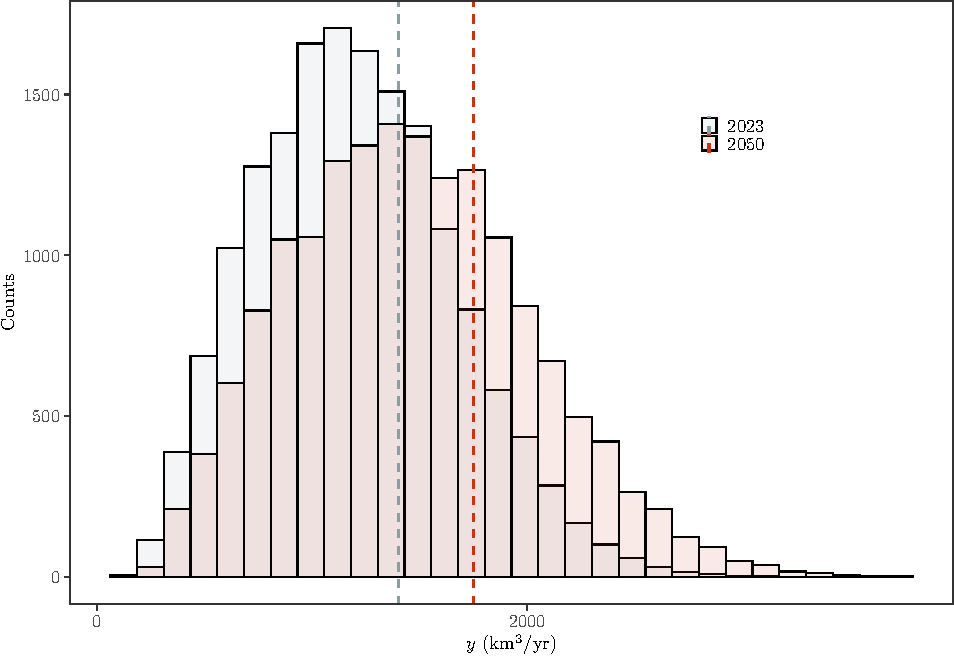
\includegraphics{code_fallacies_water_crisis_files/figure-latex/all_model-2.pdf}

\begin{Shaded}
\begin{Highlighting}[]
\CommentTok{\# Sensitivity analysis {-}{-}{-}{-}{-}{-}{-}{-}{-}{-}{-}{-}{-}{-}{-}{-}{-}{-}{-}{-}{-}{-}{-}{-}{-}{-}{-}{-}{-}{-}{-}{-}{-}{-}{-}{-}{-}{-}{-}{-}{-}{-}{-}{-}{-}{-}{-}{-}{-}{-}{-}{-}{-}{-}{-}{-}{-}}

\NormalTok{ind }\OtherTok{\textless{}{-}}\NormalTok{ dt.projections[year }\SpecialCharTok{==} \DecValTok{2023}\NormalTok{] }\SpecialCharTok{\%\textgreater{}\%}
\NormalTok{  .[, }\FunctionTok{sobol\_indices}\NormalTok{(}\AttributeTok{Y =}\NormalTok{ y, }\AttributeTok{params =}\NormalTok{ params, }\AttributeTok{N =}\NormalTok{ N, }\AttributeTok{boot =} \ConstantTok{TRUE}\NormalTok{, }\AttributeTok{R =} \DecValTok{10}\SpecialCharTok{\^{}}\DecValTok{3}\NormalTok{, }
          \AttributeTok{first =} \StringTok{"jansen"}\NormalTok{, }\AttributeTok{total =} \StringTok{"jansen"}\NormalTok{)]}
  
\NormalTok{plot.ind }\OtherTok{\textless{}{-}}\NormalTok{ ind}\SpecialCharTok{$}\NormalTok{results[parameters }\SpecialCharTok{\%in\%}\NormalTok{ params[}\DecValTok{10}\SpecialCharTok{:}\DecValTok{14}\NormalTok{]] }\SpecialCharTok{\%\textgreater{}\%}
\NormalTok{  .[}\SpecialCharTok{!}\NormalTok{parameters }\SpecialCharTok{==} \StringTok{"F\_b"}\NormalTok{] }\SpecialCharTok{\%\textgreater{}\%}
  \FunctionTok{ggplot}\NormalTok{(., }\FunctionTok{aes}\NormalTok{(parameters, original, }\AttributeTok{fill =}\NormalTok{ sensitivity)) }\SpecialCharTok{+}
  \FunctionTok{geom\_bar}\NormalTok{(}\AttributeTok{stat =} \StringTok{"identity"}\NormalTok{, }\AttributeTok{position =} \FunctionTok{position\_dodge}\NormalTok{(}\FloatTok{0.6}\NormalTok{), }\AttributeTok{color =} \StringTok{"black"}\NormalTok{) }\SpecialCharTok{+}
  \FunctionTok{scale\_y\_continuous}\NormalTok{(}\AttributeTok{breaks =} \FunctionTok{pretty\_breaks}\NormalTok{(}\AttributeTok{n =} \DecValTok{3}\NormalTok{)) }\SpecialCharTok{+}
  \FunctionTok{labs}\NormalTok{(}\AttributeTok{x =} \StringTok{""}\NormalTok{, }\AttributeTok{y =} \StringTok{"Sobol\textquotesingle{} index"}\NormalTok{) }\SpecialCharTok{+}
  \FunctionTok{geom\_errorbar}\NormalTok{(}\FunctionTok{aes}\NormalTok{(}\AttributeTok{ymin =}\NormalTok{ low.ci, }\AttributeTok{ymax =}\NormalTok{ high.ci),}
                \AttributeTok{position =} \FunctionTok{position\_dodge}\NormalTok{(}\FloatTok{0.6}\NormalTok{)) }\SpecialCharTok{+}
  \FunctionTok{scale\_fill\_discrete}\NormalTok{(}\AttributeTok{name =} \StringTok{""}\NormalTok{,}
                               \AttributeTok{labels =} \FunctionTok{c}\NormalTok{(}\FunctionTok{expression}\NormalTok{(S[}\FunctionTok{italic}\NormalTok{(i)]),}
                                          \FunctionTok{expression}\NormalTok{(T[}\FunctionTok{italic}\NormalTok{(i)]))) }\SpecialCharTok{+}
  \FunctionTok{theme\_AP}\NormalTok{() }\SpecialCharTok{+}
  \FunctionTok{theme}\NormalTok{(}\AttributeTok{legend.position =} \FunctionTok{c}\NormalTok{(}\FloatTok{0.8}\NormalTok{, }\FloatTok{0.85}\NormalTok{))}

\CommentTok{\# PLOT DISTRIBUTION OF CALORIC SUPPLY \#\#\#\#\#\#\#\#\#\#\#\#\#\#\#\#\#\#\#\#\#\#\#\#\#\#\#\#\#\#\#\#\#\#\#\#\#\#\#\#\#\#}

\NormalTok{food.fraction }\OtherTok{\textless{}{-}} \FunctionTok{fread}\NormalTok{(}\StringTok{"daily{-}per{-}capita{-}caloric{-}supply.csv"}\NormalTok{)}
\NormalTok{old\_colnames }\OtherTok{\textless{}{-}} \FunctionTok{colnames}\NormalTok{(food.fraction)}
\NormalTok{new\_colnames }\OtherTok{\textless{}{-}} \FunctionTok{c}\NormalTok{(}\StringTok{"entity"}\NormalTok{, }\StringTok{"code"}\NormalTok{, }\StringTok{"year"}\NormalTok{, }\StringTok{"kcal"}\NormalTok{)}
\FunctionTok{setnames}\NormalTok{(food.fraction, old\_colnames, new\_colnames)}
\NormalTok{plot.caloric }\OtherTok{\textless{}{-}}\NormalTok{ food.fraction[year }\SpecialCharTok{==} \DecValTok{2018}\NormalTok{] }\SpecialCharTok{\%\textgreater{}\%}
  \FunctionTok{ggplot}\NormalTok{(., }\FunctionTok{aes}\NormalTok{(kcal)) }\SpecialCharTok{+}
  \FunctionTok{geom\_histogram}\NormalTok{() }\SpecialCharTok{+} 
  \FunctionTok{scale\_x\_continuous}\NormalTok{(}\AttributeTok{breaks =} \FunctionTok{pretty\_breaks}\NormalTok{(}\AttributeTok{n =} \DecValTok{3}\NormalTok{)) }\SpecialCharTok{+}
  \FunctionTok{labs}\NormalTok{(}\AttributeTok{x =} \StringTok{"Kcal"}\NormalTok{, }\AttributeTok{y =} \StringTok{"Counts"}\NormalTok{) }\SpecialCharTok{+}
  \FunctionTok{theme\_AP}\NormalTok{()}
\end{Highlighting}
\end{Shaded}

\begin{Shaded}
\begin{Highlighting}[]
\CommentTok{\# MERGE PLOTS \#\#\#\#\#\#\#\#\#\#\#\#\#\#\#\#\#\#\#\#\#\#\#\#\#\#\#\#\#\#\#\#\#\#\#\#\#\#\#\#\#\#\#\#\#\#\#\#\#\#\#\#\#\#\#\#\#\#\#\#\#\#\#\#\#\#}

\FunctionTok{plot\_grid}\NormalTok{(plot.caloric, hist.w, hist.y, plot.ind, }\AttributeTok{ncol =} \DecValTok{2}\NormalTok{, }\AttributeTok{labels =} \StringTok{"auto"}\NormalTok{)}
\end{Highlighting}
\end{Shaded}

\begin{verbatim}
## `stat_bin()` using `bins = 30`. Pick better value with `binwidth`.
## `stat_bin()` using `bins = 30`. Pick better value with `binwidth`.
## `stat_bin()` using `bins = 30`. Pick better value with `binwidth`.
\end{verbatim}

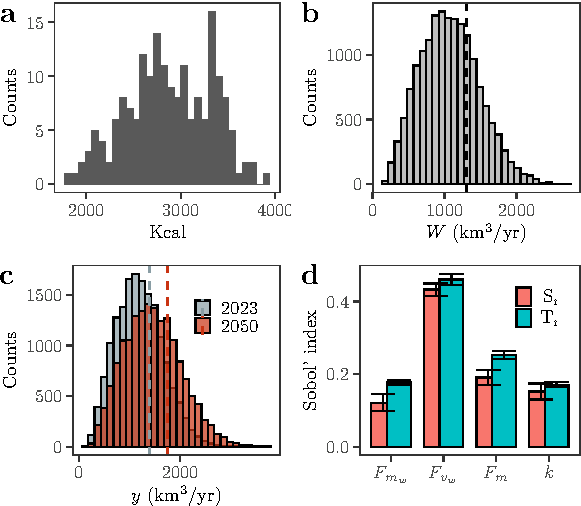
\includegraphics{code_fallacies_water_crisis_files/figure-latex/merge_figures-1.pdf}

\begin{Shaded}
\begin{Highlighting}[]
\CommentTok{\# ARRANGE DATA \#\#\#\#\#\#\#\#\#\#\#\#\#\#\#\#\#\#\#\#\#\#\#\#\#\#\#\#\#\#\#\#\#\#\#\#\#\#\#\#\#\#\#\#\#\#\#\#\#\#\#\#\#\#\#\#\#\#\#\#\#\#\#\#\#}

\NormalTok{tmp }\OtherTok{\textless{}{-}} \FunctionTok{split}\NormalTok{(dt.projections, dt.projections}\SpecialCharTok{$}\NormalTok{year) }\SpecialCharTok{\%\textgreater{}\%}
  \FunctionTok{lapply}\NormalTok{(., }\ControlFlowTok{function}\NormalTok{(x) x[, }\AttributeTok{year:=} \ConstantTok{NULL}\NormalTok{])}

\NormalTok{years }\OtherTok{\textless{}{-}} \FunctionTok{c}\NormalTok{(}\DecValTok{2023}\NormalTok{, }\DecValTok{2050}\NormalTok{)}

\NormalTok{out }\OtherTok{\textless{}{-}} \FunctionTok{list}\NormalTok{()}
\ControlFlowTok{for}\NormalTok{(i }\ControlFlowTok{in} \DecValTok{1}\SpecialCharTok{:}\FunctionTok{length}\NormalTok{(tmp)) \{}
  
\NormalTok{  out[[i]] }\OtherTok{\textless{}{-}} \FunctionTok{setnames}\NormalTok{(tmp[[i]], }\FunctionTok{colnames}\NormalTok{(tmp[[i]]), }
                       \FunctionTok{paste}\NormalTok{(}\FunctionTok{colnames}\NormalTok{(tmp[[i]]), years[[i]], }\AttributeTok{sep =} \StringTok{"."}\NormalTok{))}
  
  
\NormalTok{\}}
  
\NormalTok{dt }\OtherTok{\textless{}{-}} \FunctionTok{do.call}\NormalTok{(cbind, out) }\SpecialCharTok{\%\textgreater{}\%}
  \FunctionTok{cbind}\NormalTok{(land\_runoff, exceedance\_2023, .) }\SpecialCharTok{\%\textgreater{}\%}
\NormalTok{  .[}\DecValTok{1}\SpecialCharTok{:}\NormalTok{(}\DecValTok{2} \SpecialCharTok{*}\NormalTok{ N)] }\SpecialCharTok{\%\textgreater{}\%}
\NormalTok{  .[, outside}\SpecialCharTok{:=} \FunctionTok{ifelse}\NormalTok{(land\_runoff }\SpecialCharTok{\textless{}}\NormalTok{ land\_runoff\_min }\SpecialCharTok{|}
\NormalTok{                         land\_runoff }\SpecialCharTok{\textgreater{}}\NormalTok{ land\_runoff\_max, }\StringTok{"Yes"}\NormalTok{, }\StringTok{"No"}\NormalTok{)] }\SpecialCharTok{\%\textgreater{}\%}
\NormalTok{  .[, accessible\_water\_runoff}\SpecialCharTok{:=}\NormalTok{ land\_runoff }\SpecialCharTok{{-}} \DecValTok{7800} \SpecialCharTok{{-}} \DecValTok{20400}\NormalTok{] }\SpecialCharTok{\%\textgreater{}\%}
\NormalTok{  .[, outside\_runoff}\SpecialCharTok{:=} \FunctionTok{ifelse}\NormalTok{(accessible\_water\_runoff }\SpecialCharTok{\textless{}} \DecValTok{12500} \SpecialCharTok{|} 
\NormalTok{                                accessible\_water\_runoff }\SpecialCharTok{\textgreater{}} \DecValTok{18500}\NormalTok{, }\StringTok{"Yes"}\NormalTok{, }\StringTok{"No"}\NormalTok{)] }\SpecialCharTok{\%\textgreater{}\%}
\NormalTok{  .[, water\_deficit}\SpecialCharTok{:=} \FunctionTok{ifelse}\NormalTok{(exceedance\_2023 }\SpecialCharTok{\textgreater{}} \DecValTok{0}\NormalTok{, }\StringTok{"Yes"}\NormalTok{, }\StringTok{"No"}\NormalTok{)]}

\NormalTok{dt }\OtherTok{\textless{}{-}}\NormalTok{ dt[, additional\_water\_2050}\SpecialCharTok{:=}\NormalTok{ y}\FloatTok{.2050} \SpecialCharTok{{-}}\NormalTok{ y}\FloatTok{.2023}\NormalTok{] }\SpecialCharTok{\%\textgreater{}\%}
\NormalTok{  .[, exceedance\_2050}\SpecialCharTok{:=}\NormalTok{ exceedance\_2023 }\SpecialCharTok{+}\NormalTok{ additional\_water\_2050] }\SpecialCharTok{\%\textgreater{}\%}
\NormalTok{  .[, exceedance\_by\_2050}\SpecialCharTok{:=} \FunctionTok{ifelse}\NormalTok{(exceedance\_2050 }\SpecialCharTok{\textgreater{}} \DecValTok{0}\NormalTok{, }\StringTok{"Yes"}\NormalTok{, }\StringTok{"No"}\NormalTok{)]}

\CommentTok{\# SOME STATS \#\#\#\#\#\#\#\#\#\#\#\#\#\#\#\#\#\#\#\#\#\#\#\#\#\#\#\#\#\#\#\#\#\#\#\#\#\#\#\#\#\#\#\#\#\#\#\#\#\#\#\#\#\#\#\#\#\#\#\#\#\#\#\#\#\#\#}

\NormalTok{cols }\OtherTok{\textless{}{-}} \FunctionTok{c}\NormalTok{(}\StringTok{"land\_runoff"}\NormalTok{, }\StringTok{"accessible\_water\_runoff"}\NormalTok{, }\StringTok{"exceedance\_2023"}\NormalTok{)}
\NormalTok{summary\_fun }\OtherTok{=} \ControlFlowTok{function}\NormalTok{(x) }\FunctionTok{list}\NormalTok{(}\AttributeTok{min =} \FunctionTok{min}\NormalTok{(x), }\AttributeTok{max =} \FunctionTok{max}\NormalTok{(x))}
\NormalTok{dt[, }\FunctionTok{lapply}\NormalTok{(.SD, summary\_fun), .SDcols }\OtherTok{=}\NormalTok{ (cols)]}
\end{Highlighting}
\end{Shaded}

\begin{verbatim}
##    land_runoff accessible_water_runoff exceedance_2023
## 1:    33441.89                5241.895       -2593.442
## 2:    58552.83                30352.83        1333.539
\end{verbatim}

\begin{Shaded}
\begin{Highlighting}[]
\NormalTok{tmp }\OtherTok{\textless{}{-}} \FunctionTok{melt}\NormalTok{(dt, }\AttributeTok{measure.vars =} \FunctionTok{c}\NormalTok{(}\StringTok{"outside"}\NormalTok{, }\StringTok{"outside\_runoff"}\NormalTok{, }\StringTok{"water\_deficit"}\NormalTok{)) }\SpecialCharTok{\%\textgreater{}\%}
\NormalTok{  .[, .N, .(variable, value)]}

\NormalTok{tmp[, total}\SpecialCharTok{:=}\NormalTok{ (}\DecValTok{2}\SpecialCharTok{\^{}}\DecValTok{13} \SpecialCharTok{*} \DecValTok{2}\NormalTok{)] }\SpecialCharTok{\%\textgreater{}\%}
\NormalTok{  .[, prop}\SpecialCharTok{:=}\NormalTok{ N }\SpecialCharTok{/}\NormalTok{ total] }\SpecialCharTok{\%\textgreater{}\%}
  \FunctionTok{print}\NormalTok{()}
\end{Highlighting}
\end{Shaded}

\begin{verbatim}
##          variable value     N total      prop
## 1:        outside    No  6275 16384 0.3829956
## 2:        outside   Yes 10109 16384 0.6170044
## 3: outside_runoff    No  4089 16384 0.2495728
## 4: outside_runoff   Yes 12295 16384 0.7504272
## 5:  water_deficit    No 12571 16384 0.7672729
## 6:  water_deficit   Yes  3813 16384 0.2327271
\end{verbatim}

\begin{Shaded}
\begin{Highlighting}[]
\CommentTok{\# PLOT LAND RUNOFF DISTRIBUTION \#\#\#\#\#\#\#\#\#\#\#\#\#\#\#\#\#\#\#\#\#\#\#\#\#\#\#\#\#\#\#\#\#\#\#\#\#\#\#\#\#\#\#\#\#\#\#\#}

\NormalTok{plot\_land\_runoff }\OtherTok{\textless{}{-}} \FunctionTok{ggplot}\NormalTok{(dt, }\FunctionTok{aes}\NormalTok{(land\_runoff, }\AttributeTok{fill =}\NormalTok{ outside)) }\SpecialCharTok{+}
  \FunctionTok{geom\_histogram}\NormalTok{(}\AttributeTok{colour =} \StringTok{"black"}\NormalTok{) }\SpecialCharTok{+}
  \FunctionTok{scale\_fill\_manual}\NormalTok{(}\AttributeTok{values =} \FunctionTok{c}\NormalTok{(}\StringTok{"white"}\NormalTok{, }\StringTok{"grey"}\NormalTok{)) }\SpecialCharTok{+}
  \FunctionTok{theme\_AP}\NormalTok{() }\SpecialCharTok{+} 
  \FunctionTok{geom\_vline}\NormalTok{(}\AttributeTok{xintercept =}\NormalTok{ land\_runoff\_estimate, }\AttributeTok{color =} \StringTok{"red"}\NormalTok{, }\AttributeTok{lty =} \DecValTok{2}\NormalTok{, }\AttributeTok{size =} \DecValTok{2}\NormalTok{) }\SpecialCharTok{+}
  \FunctionTok{labs}\NormalTok{(}\AttributeTok{x =} \StringTok{"Global land runoff }\SpecialCharTok{\textbackslash{}n}\StringTok{ (km$\^{}3$/year)"}\NormalTok{, }\AttributeTok{y =} \StringTok{"Counts"}\NormalTok{) }\SpecialCharTok{+}
  \FunctionTok{theme}\NormalTok{(}\AttributeTok{legend.position =} \StringTok{"none"}\NormalTok{)}

\NormalTok{plot\_land\_runoff}
\end{Highlighting}
\end{Shaded}

\begin{verbatim}
## `stat_bin()` using `bins = 30`. Pick better value with `binwidth`.
\end{verbatim}

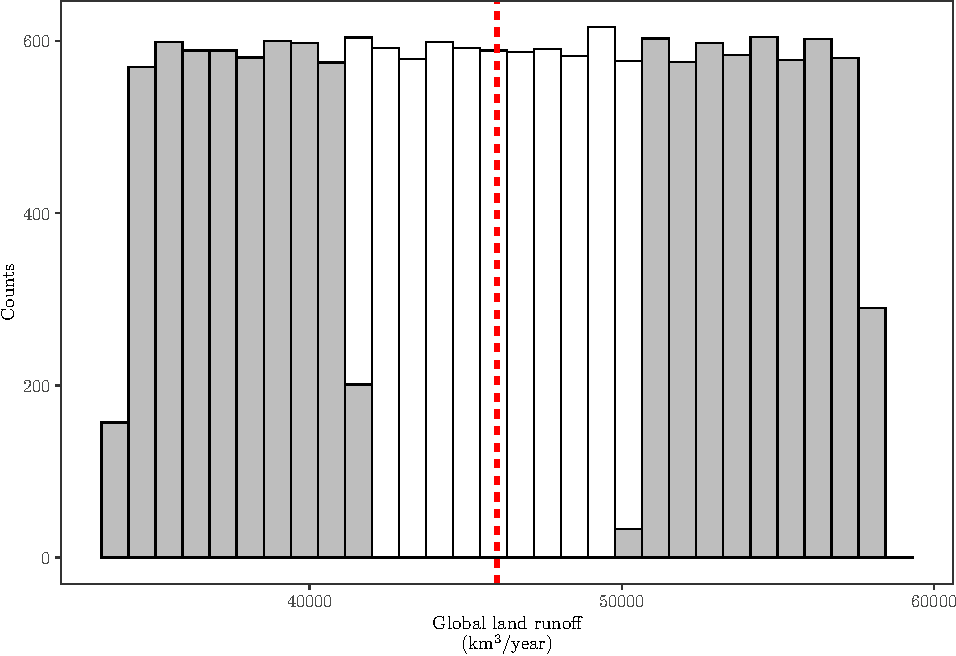
\includegraphics{code_fallacies_water_crisis_files/figure-latex/rest-1.pdf}

\begin{Shaded}
\begin{Highlighting}[]
\CommentTok{\# PLOT ACCESSIBLE RUNOFF \#\#\#\#\#\#\#\#\#\#\#\#\#\#\#\#\#\#\#\#\#\#\#\#\#\#\#\#\#\#\#\#\#\#\#\#\#\#\#\#\#\#\#\#\#\#\#\#\#\#\#\#\#\#\#}

\NormalTok{plot\_accessible\_runoff }\OtherTok{\textless{}{-}} \FunctionTok{ggplot}\NormalTok{(dt, }\FunctionTok{aes}\NormalTok{(accessible\_water\_runoff, }\AttributeTok{fill =}\NormalTok{ outside\_runoff)) }\SpecialCharTok{+}
  \FunctionTok{geom\_histogram}\NormalTok{(}\AttributeTok{colour =} \StringTok{"black"}\NormalTok{) }\SpecialCharTok{+}
  \FunctionTok{scale\_fill\_manual}\NormalTok{(}\AttributeTok{values =} \FunctionTok{c}\NormalTok{(}\StringTok{"white"}\NormalTok{, }\StringTok{"grey"}\NormalTok{)) }\SpecialCharTok{+}
  \FunctionTok{theme\_AP}\NormalTok{() }\SpecialCharTok{+} 
  \FunctionTok{labs}\NormalTok{(}\AttributeTok{x =} \StringTok{"Accessible blue water runoff }\SpecialCharTok{\textbackslash{}n}\StringTok{ (km$\^{}3$/year)"}\NormalTok{, }\AttributeTok{y =} \StringTok{""}\NormalTok{) }\SpecialCharTok{+}
  \FunctionTok{theme}\NormalTok{(}\AttributeTok{legend.position =} \StringTok{"none"}\NormalTok{)}

\NormalTok{plot\_accessible\_runoff}
\end{Highlighting}
\end{Shaded}

\begin{verbatim}
## `stat_bin()` using `bins = 30`. Pick better value with `binwidth`.
\end{verbatim}

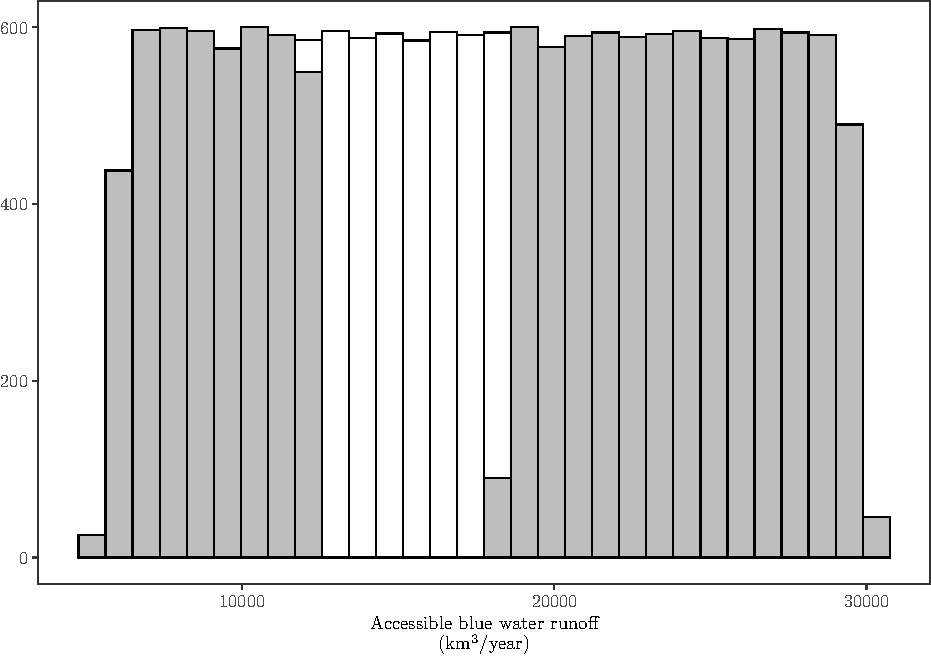
\includegraphics{code_fallacies_water_crisis_files/figure-latex/rest-2.pdf}

\begin{Shaded}
\begin{Highlighting}[]
\CommentTok{\# PLOT ACCESSIBLE BLUE WATER RUNOFF CONSUMES BY IRRIGATION \#\#\#\#\#\#\#\#\#\#\#\#\#\#\#\#\#\#\#\#\#}

\NormalTok{vec }\OtherTok{\textless{}{-}} \FunctionTok{data.table}\NormalTok{(}\AttributeTok{fraction.irrig =} \DecValTok{1600} \SpecialCharTok{/}\NormalTok{ dt}\SpecialCharTok{$}\NormalTok{accessible\_water\_runoff)}

\NormalTok{plot.irrigation }\OtherTok{\textless{}{-}} \FunctionTok{ggplot}\NormalTok{(vec, }\FunctionTok{aes}\NormalTok{(fraction.irrig)) }\SpecialCharTok{+}
  \FunctionTok{geom\_histogram}\NormalTok{(}\AttributeTok{fill =} \StringTok{"grey"}\NormalTok{, }\AttributeTok{color =} \StringTok{"black"}\NormalTok{) }\SpecialCharTok{+} 
  \FunctionTok{labs}\NormalTok{(}\AttributeTok{x =} \StringTok{"Fraction consumed }\SpecialCharTok{\textbackslash{}n}\StringTok{ by irrigation"}\NormalTok{, }\AttributeTok{y =} \StringTok{""}\NormalTok{) }\SpecialCharTok{+}
  \FunctionTok{theme\_AP}\NormalTok{()}

\NormalTok{plot.irrigation}
\end{Highlighting}
\end{Shaded}

\begin{verbatim}
## `stat_bin()` using `bins = 30`. Pick better value with `binwidth`.
\end{verbatim}

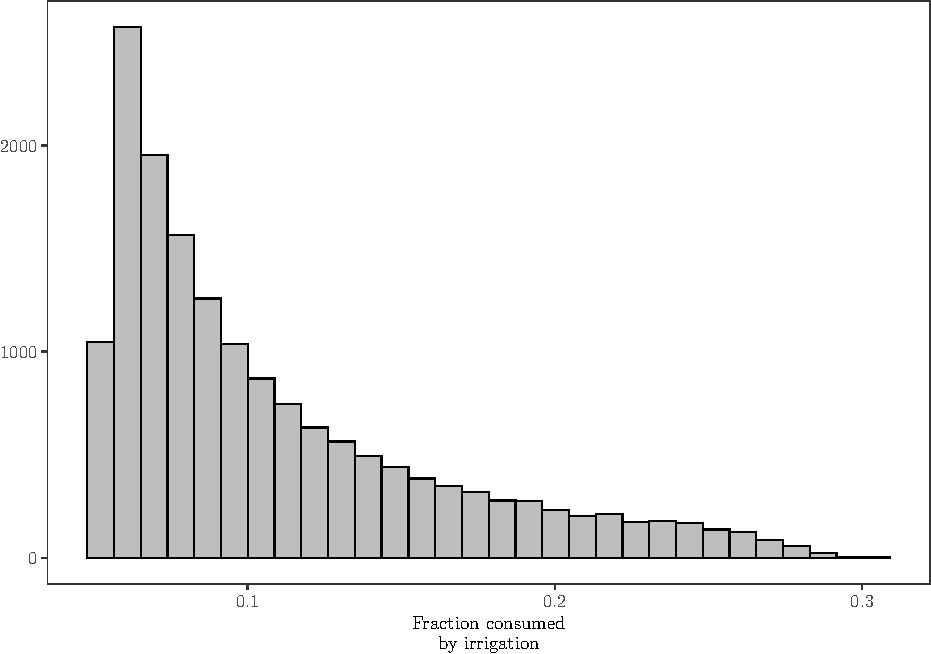
\includegraphics{code_fallacies_water_crisis_files/figure-latex/rest-3.pdf}

\begin{Shaded}
\begin{Highlighting}[]
\CommentTok{\# FRACTION OF IRRIGATION SUPPLIED BY SURFACE WATER \#\#\#\#\#\#\#\#\#\#\#\#\#\#\#\#\#\#\#\#\#\#\#\#\#\#\#\#\#}

\NormalTok{da }\OtherTok{\textless{}{-}} \FunctionTok{data.table}\NormalTok{(readxl}\SpecialCharTok{::}\FunctionTok{read\_xls}\NormalTok{(}\StringTok{"/Users/arnaldpuy/Documents/papers/fallacies\_water\_crisis/code\_fallacies\_water\_crisis/HESS\_2010\_159\_Supplement\_S2.xls"}\NormalTok{))}
\NormalTok{da }\OtherTok{\textless{}{-}}\NormalTok{ da[, fraction.gw}\SpecialCharTok{:=} \StringTok{\textasciigrave{}}\AttributeTok{ICU\_GW (m3 yr{-}1)}\StringTok{\textasciigrave{}} \SpecialCharTok{/} \StringTok{\textasciigrave{}}\AttributeTok{ICU (m3 yr{-}1)}\StringTok{\textasciigrave{}}\NormalTok{] }\SpecialCharTok{\%\textgreater{}\%}
\NormalTok{  .[, fraction.irr}\SpecialCharTok{:=} \StringTok{\textasciigrave{}}\AttributeTok{ICU\_SW (m3 yr{-}1)}\StringTok{\textasciigrave{}} \SpecialCharTok{/} \StringTok{\textasciigrave{}}\AttributeTok{ICU (m3 yr{-}1)}\StringTok{\textasciigrave{}}\NormalTok{]}


\NormalTok{da[fraction.irr }\SpecialCharTok{\textless{}} \FloatTok{0.05}\NormalTok{] }\SpecialCharTok{\%\textgreater{}\%}
\NormalTok{  .[, .(COUNTRY, fraction.irr, fraction.gw)]}
\end{Highlighting}
\end{Shaded}

\begin{verbatim}
##                            COUNTRY fraction.irr fraction.gw
##  1:                        Bahrain  0.000000000   0.9031133
##  2:                        Denmark  0.000000000   1.0000000
##  3:                       Djibouti  0.000000000   1.0000000
##  4:                         Kuwait  0.000000000   0.6100000
##  5:         Libyan Arab Jamahiriya  0.005554530   0.9888909
##  6:                          Malta  0.005586855   0.9944131
##  7:                     Montenegro  0.003619909   0.9963801
##  8: Occupied Palestinian Territory  0.000000000   1.0000000
##  9:                           Oman  0.000000000   1.0000000
## 10:                          Qatar  0.000000000   0.9339782
## 11:                   Saudi Arabia  0.000000000   0.9700133
## 12:           United Arab Emirates  0.000000000   1.0000000
\end{verbatim}

\begin{Shaded}
\begin{Highlighting}[]
\NormalTok{fraction.surface }\OtherTok{\textless{}{-}} \FunctionTok{ggplot}\NormalTok{(da, }\FunctionTok{aes}\NormalTok{(fraction.irr)) }\SpecialCharTok{+}
  \FunctionTok{geom\_histogram}\NormalTok{(}\AttributeTok{color =} \StringTok{"black"}\NormalTok{, }\AttributeTok{fill =} \StringTok{"grey"}\NormalTok{) }\SpecialCharTok{+} 
  \FunctionTok{theme\_AP}\NormalTok{() }\SpecialCharTok{+} 
  \FunctionTok{geom\_vline}\NormalTok{(}\AttributeTok{xintercept =} \FloatTok{0.71}\NormalTok{, }\AttributeTok{lty =} \DecValTok{2}\NormalTok{) }\SpecialCharTok{+} 
  \FunctionTok{labs}\NormalTok{(}\AttributeTok{x =} \StringTok{"Fraction of surface water"}\NormalTok{, }\AttributeTok{y =} \StringTok{"Nº countries"}\NormalTok{)}

\NormalTok{fraction.surface}
\end{Highlighting}
\end{Shaded}

\begin{verbatim}
## `stat_bin()` using `bins = 30`. Pick better value with `binwidth`.
\end{verbatim}

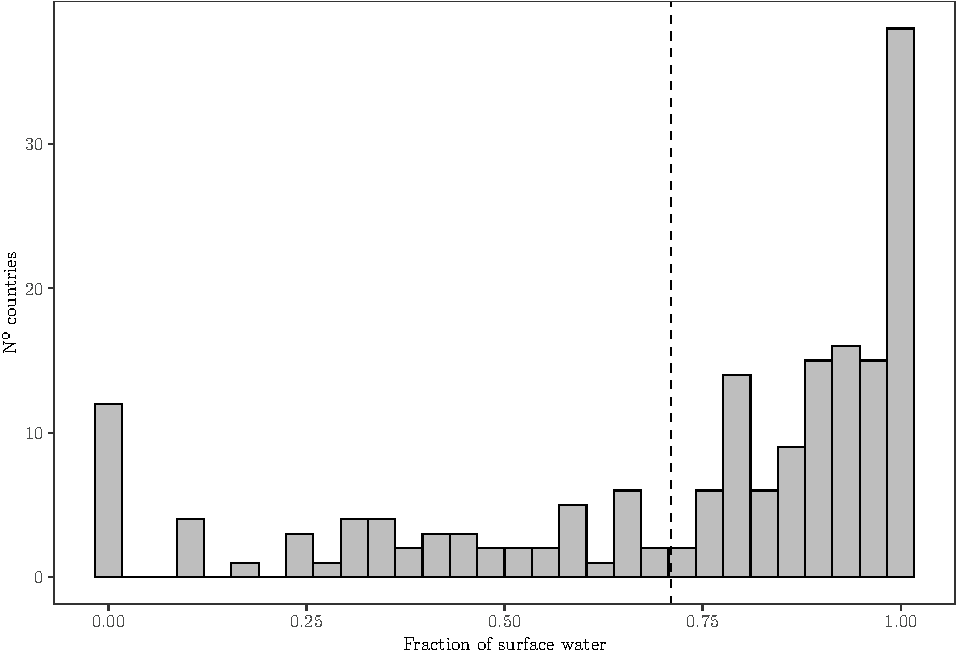
\includegraphics{code_fallacies_water_crisis_files/figure-latex/rest-4.pdf}

\begin{Shaded}
\begin{Highlighting}[]
\CommentTok{\# PLOT CORRECTED WATER LIMIT EXCEEDANCE FOR 2023 \#\#\#\#\#\#\#\#\#\#\#\#\#\#\#\#\#\#\#\#\#\#\#\#\#\#\#\#\#\#}

\NormalTok{plot.exceedance }\OtherTok{\textless{}{-}} \FunctionTok{ggplot}\NormalTok{(dt, }\FunctionTok{aes}\NormalTok{(exceedance\_2023, }\AttributeTok{fill =}\NormalTok{ water\_deficit)) }\SpecialCharTok{+}
  \FunctionTok{geom\_histogram}\NormalTok{(}\AttributeTok{color =} \StringTok{"black"}\NormalTok{) }\SpecialCharTok{+}
  \FunctionTok{scale\_fill\_manual}\NormalTok{(}\AttributeTok{values =} \FunctionTok{c}\NormalTok{(}\StringTok{"grey"}\NormalTok{, }\StringTok{"\#F8766D"}\NormalTok{), }
                    \AttributeTok{name =} \StringTok{"Water }\SpecialCharTok{\textbackslash{}n}\StringTok{ exceedance"}\NormalTok{) }\SpecialCharTok{+}
  \FunctionTok{scale\_x\_continuous}\NormalTok{(}\AttributeTok{breaks =} \FunctionTok{pretty\_breaks}\NormalTok{(}\AttributeTok{n =} \DecValTok{2}\NormalTok{)) }\SpecialCharTok{+}
  \FunctionTok{labs}\NormalTok{(}\AttributeTok{x =} \StringTok{"km$\^{}3$/yr"}\NormalTok{, }\AttributeTok{y =} \StringTok{"Counts"}\NormalTok{) }\SpecialCharTok{+}
  \FunctionTok{geom\_vline}\NormalTok{(}\AttributeTok{xintercept =} \FloatTok{287.5}\NormalTok{, }\AttributeTok{lty =} \DecValTok{2}\NormalTok{) }\SpecialCharTok{+}
  \FunctionTok{theme\_AP}\NormalTok{() }\SpecialCharTok{+}
  \FunctionTok{theme}\NormalTok{(}\AttributeTok{legend.position =} \FunctionTok{c}\NormalTok{(}\FloatTok{0.22}\NormalTok{, }\FloatTok{0.73}\NormalTok{))}

\NormalTok{plot.exceedance}
\end{Highlighting}
\end{Shaded}

\begin{verbatim}
## `stat_bin()` using `bins = 30`. Pick better value with `binwidth`.
\end{verbatim}

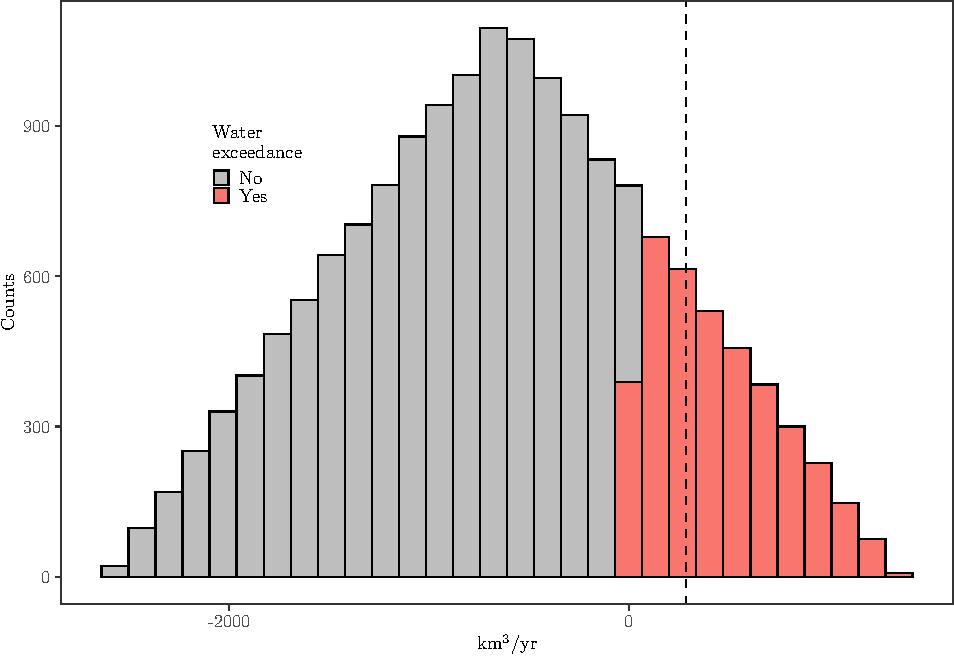
\includegraphics{code_fallacies_water_crisis_files/figure-latex/rest-5.pdf}

\begin{Shaded}
\begin{Highlighting}[]
\CommentTok{\# PLOT WATER EXCEEDANCE IN 2025 \#\#\#\#\#\#\#\#\#\#\#\#\#\#\#\#\#\#\#\#\#\#\#\#\#\#\#\#\#\#\#\#\#\#\#\#\#\#\#\#\#\#\#\#\#\#\#\#}

\NormalTok{plot.exceedance}\FloatTok{.2050} \OtherTok{\textless{}{-}} \FunctionTok{ggplot}\NormalTok{(dt, }\FunctionTok{aes}\NormalTok{(exceedance\_2050, }\AttributeTok{fill =}\NormalTok{ exceedance\_by\_2050)) }\SpecialCharTok{+}
  \FunctionTok{geom\_histogram}\NormalTok{(}\AttributeTok{color =} \StringTok{"black"}\NormalTok{) }\SpecialCharTok{+}
  \FunctionTok{scale\_fill\_manual}\NormalTok{(}\AttributeTok{values =} \FunctionTok{c}\NormalTok{(}\StringTok{"grey"}\NormalTok{, }\StringTok{"\#F8766D"}\NormalTok{), }
                    \AttributeTok{name =} \StringTok{"Water }\SpecialCharTok{\textbackslash{}n}\StringTok{ exceedance"}\NormalTok{) }\SpecialCharTok{+}
  \FunctionTok{scale\_x\_continuous}\NormalTok{(}\AttributeTok{breaks =} \FunctionTok{pretty\_breaks}\NormalTok{(}\AttributeTok{n =} \DecValTok{2}\NormalTok{)) }\SpecialCharTok{+}
  \FunctionTok{geom\_vline}\NormalTok{(}\AttributeTok{xintercept =} \FloatTok{627.5}\NormalTok{, }\AttributeTok{lty =} \DecValTok{2}\NormalTok{) }\SpecialCharTok{+}
  \FunctionTok{labs}\NormalTok{(}\AttributeTok{x =} \StringTok{"km$\^{}3$/yr"}\NormalTok{, }\AttributeTok{y =} \StringTok{"Counts"}\NormalTok{) }\SpecialCharTok{+}
  \FunctionTok{theme\_AP}\NormalTok{() }

\NormalTok{plot.exceedance}\FloatTok{.2050}
\end{Highlighting}
\end{Shaded}

\begin{verbatim}
## `stat_bin()` using `bins = 30`. Pick better value with `binwidth`.
\end{verbatim}

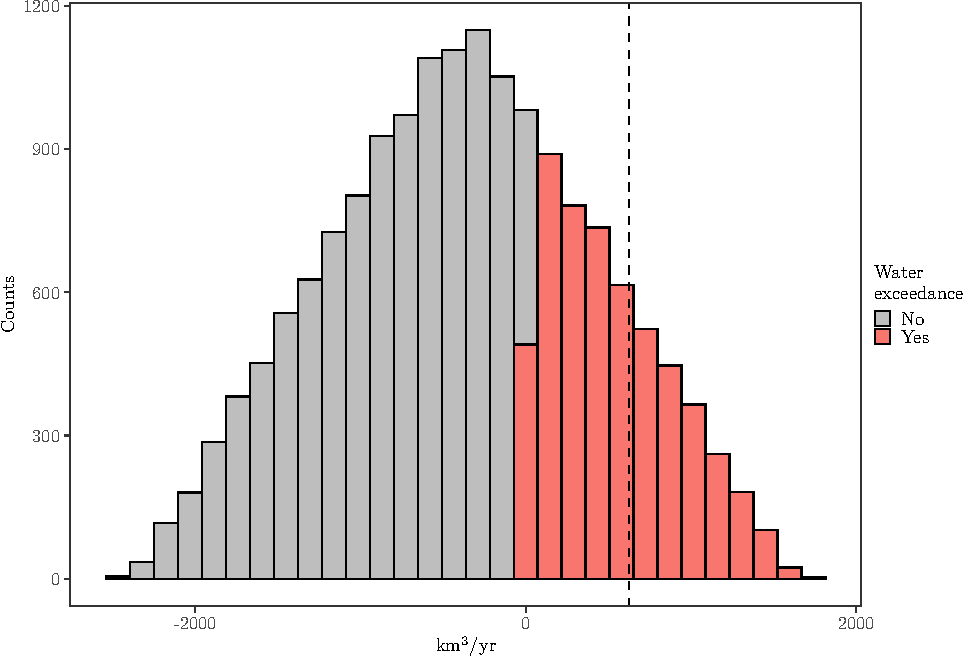
\includegraphics{code_fallacies_water_crisis_files/figure-latex/rest-6.pdf}

\begin{Shaded}
\begin{Highlighting}[]
\CommentTok{\# MERGE PLOTS \#\#\#\#\#\#\#\#\#\#\#\#\#\#\#\#\#\#\#\#\#\#\#\#\#\#\#\#\#\#\#\#\#\#\#\#\#\#\#\#\#\#\#\#\#\#\#\#\#\#\#\#\#\#\#\#\#\#\#\#\#\#\#\#\#\#}

\NormalTok{top }\OtherTok{\textless{}{-}} \FunctionTok{plot\_grid}\NormalTok{(plot\_land\_runoff, plot\_accessible\_runoff, plot.irrigation, }
                 \AttributeTok{labels =} \FunctionTok{c}\NormalTok{(}\StringTok{"a"}\NormalTok{, }\StringTok{""}\NormalTok{, }\StringTok{"b"}\NormalTok{), }\AttributeTok{rel\_widths =} \FunctionTok{c}\NormalTok{(}\FloatTok{0.34}\NormalTok{, }\FloatTok{0.32}\NormalTok{, }\FloatTok{0.32}\NormalTok{), }\AttributeTok{ncol =} \DecValTok{3}\NormalTok{)}
\end{Highlighting}
\end{Shaded}

\begin{verbatim}
## `stat_bin()` using `bins = 30`. Pick better value with `binwidth`.
## `stat_bin()` using `bins = 30`. Pick better value with `binwidth`.
## `stat_bin()` using `bins = 30`. Pick better value with `binwidth`.
\end{verbatim}

\begin{Shaded}
\begin{Highlighting}[]
\NormalTok{bottom }\OtherTok{\textless{}{-}} \FunctionTok{plot\_grid}\NormalTok{(fraction.surface, plot.exceedance }\SpecialCharTok{+} 
                      \FunctionTok{theme}\NormalTok{(}\AttributeTok{legend.position =} \StringTok{"none"}\NormalTok{), plot.exceedance}\FloatTok{.2050}\NormalTok{, }
                    \AttributeTok{labels =} \FunctionTok{c}\NormalTok{(}\StringTok{"c"}\NormalTok{, }\StringTok{"d"}\NormalTok{, }\StringTok{"e"}\NormalTok{), }\AttributeTok{rel\_widths =} \FunctionTok{c}\NormalTok{(}\FloatTok{0.30}\NormalTok{, }\FloatTok{0.305}\NormalTok{, }\FloatTok{0.425}\NormalTok{), }\AttributeTok{ncol =} \DecValTok{3}\NormalTok{)}
\end{Highlighting}
\end{Shaded}

\begin{verbatim}
## `stat_bin()` using `bins = 30`. Pick better value with `binwidth`.
## `stat_bin()` using `bins = 30`. Pick better value with `binwidth`.
## `stat_bin()` using `bins = 30`. Pick better value with `binwidth`.
\end{verbatim}

\begin{Shaded}
\begin{Highlighting}[]
\FunctionTok{plot\_grid}\NormalTok{(top, bottom, }\AttributeTok{ncol =} \DecValTok{1}\NormalTok{)}
\end{Highlighting}
\end{Shaded}

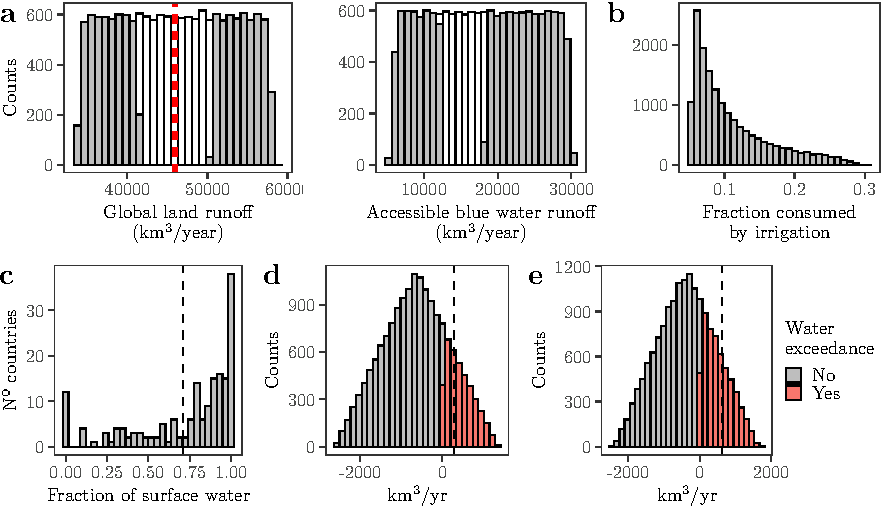
\includegraphics{code_fallacies_water_crisis_files/figure-latex/merge_plots-1.pdf}

\newpage

\end{document}
